\subsubsection{3.3V Speisung}
\label{subsubsec:3.3V Speisung}

Um die Treiber der Motorenansteuerung, das Wirelessmodul und die RFID-Schaltung betreiben zu können, wird zusätzlich eine 3,3V Speisung verbaut. Da es sich dabei nicht um enorm Leistungstreibende Elemente handelt, wurde entschieden einen einfachen Linearregler einzusetzen, welcher von der 5V Speisung aus betrieben wird. 

\paragraph{Schema}\mbox{}\\

Bei dem Linearregler handelt es sich konkret um den LF33CDT-TRY von STMicroelectronics. Dieser hat eine fixe Ausgangsspannung von 3.3V, bei einem maximalen Strom von 1A. Das dazugehörige Schama kann in Abbildung \ref{fig:Schema_Speisung_3.3V} begutachtet werden. \cite{stmicroelectronics_lf33cdt-try_2017}

\begin{figure}[h!]
	\centering
	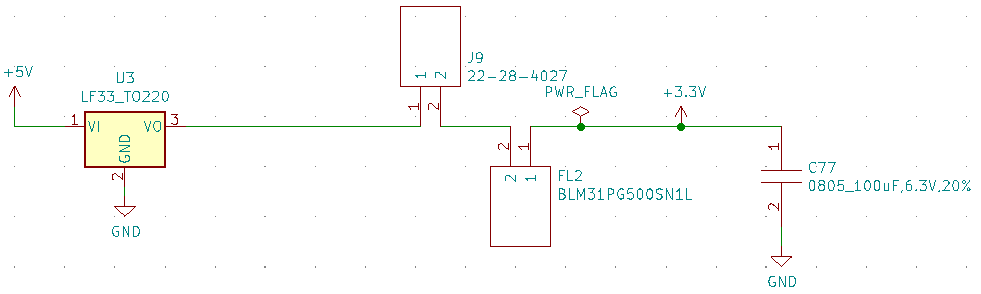
\includegraphics[width=0.5\textwidth]{graphics/Schema_Speisung_3,3V.png}
	\caption{Schema der 3.3V Speisung}
	\label{fig:Schema_Speisung_3.3V}
\end{figure} 


\paragraph{Funktionsbeschrieb der Schaltung}\mbox{}\\

Der Linearregler benötigt keine spezielle Beschaltung. Er wird lediglich an die 5V Speisung angeschlossen. Am Eingang und am Ausgang ist ein Entstörkondensator implementiert. 

Wie bei der 12V Speisung in Kapitel \ref{subsubsec:12V Speisung} und der 5V Speisung in \ref{subsubsec:5V Speisung} wurde ein Jumper, sowie zwei LED's zu Testzwecken implementiert und auch hier Filtert ein Ferrit FL1 letzte Störungen heraus.